\section{Proposed Framework}
\label{sec:framework}

In this section, we explain our framework to solve the energy
optimization problem described in the last section. The input to the
framework is as follows: A streaming application, which is represented
as a task graph with N tasks $\textless T_{1}, T_{2}, ..., T_{N}
\textgreater$, $M_{i}$ sets of custom instructions for the task $T_i
\textless CI_{i1}, ..., CI_{iM}\textgreater$, V levels of available
voltages/frequencies $\textless vf_{1}, ..., vf_{V}\textgreater$ and C
cache configurations $\textless Ca_{1}, ..., Ca_{C}\textgreater$. The
designer provides the steady state \textit{period} constraint, $P_{c}
$, and the \textit{area} constraint, $A_{c}$ as the input constraints
to the framework. Figure \ref{fig:framework} shows the flow of the
framework. In the profiling stage, we profile the differing sets of
custom instructions of the individual tasks on a single PE at differing
voltage/frequency levels and with differing cache configurations to
obtain latencies and energy consumptions of their single iterations. For
instance, for task $T_{i}$, $M_{i} \times V \times C$ simulations are
run to capture latency and energy consumption of every implementation
of $T_{i}$ on a single PE. Additionally, we collect the trace of each
simulation during the profiling stage. The second stage, named latency-
energy estimation, is then used to analytically estimate the latency
and energy consumption of differing mappings of the tasks on the PEs
using the profiling information and traces generated by the first stage.
Lastly, the framework uses a novel branch and bound algorithm based upon
the estimation performed by the second stage to quickly and efficiently
prune and search the design space for the optimal design point -- the one
with minimum energy consumption.

\begin{figure}[h]
\center
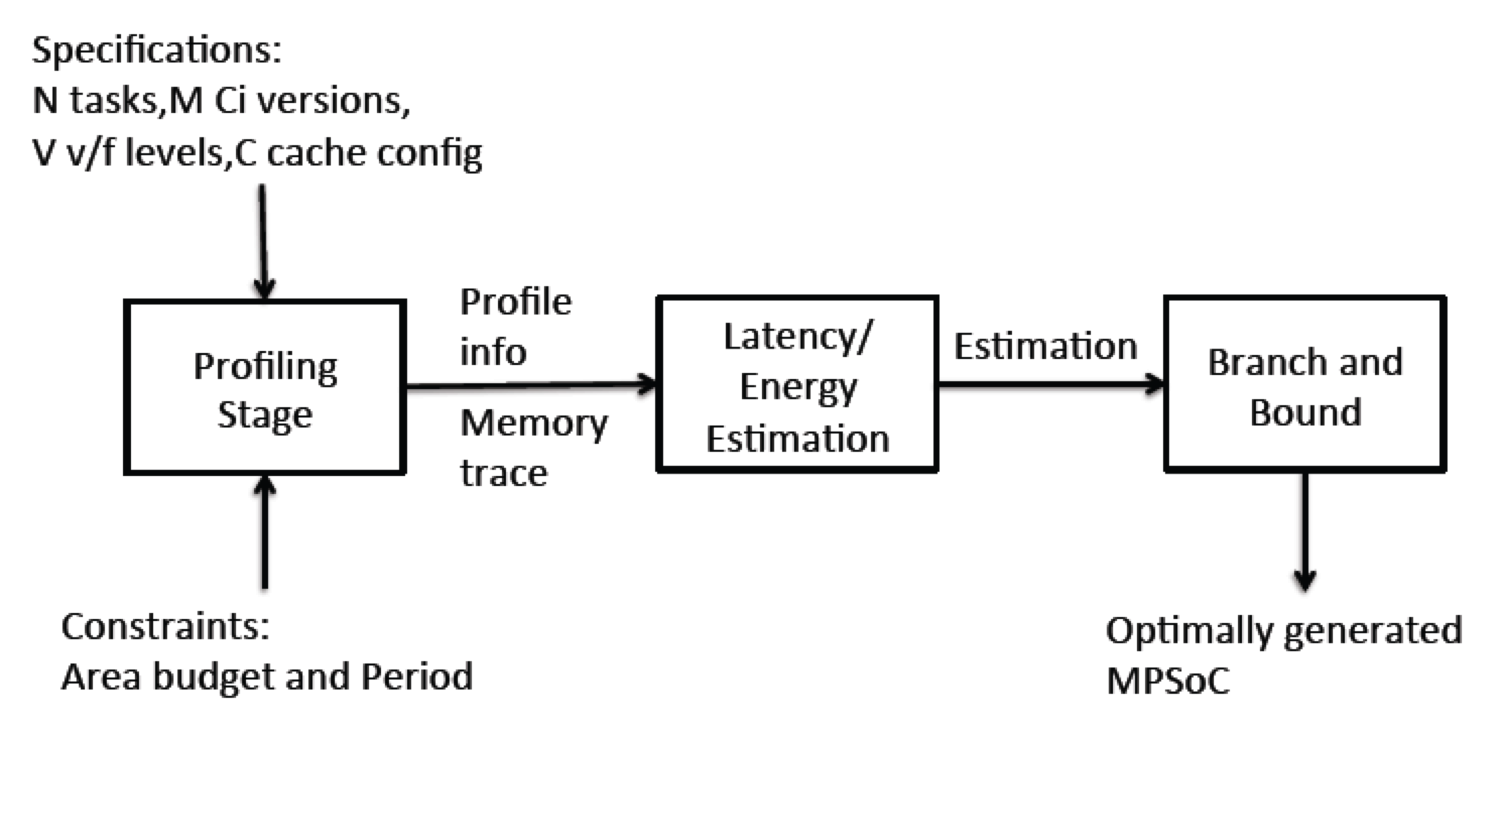
\includegraphics[width=0.40\textwidth, height=0.27\textwidth]{framework.png}
\label{fig:framework}
\caption {Framework Flow}
\end{figure}

\subsection{Latency-Energy Estimation}

As mentioned earlier, we use general task mapping as it allows greater
flexibility and efficiency in terms of energy. Generating all the possible task mappings
is equivalent to enumerating all the possible set partitions~\cite{}.
For example, an application, consisting of five tasks, can be mapped
onto five PEs in 52 different ways (some PEs might not have any task
mapped on them). It is not realistic to simulate all the possible
mappings of all the tasks when the number of tasks increases. This is
further exacerbated by the availability of differing custom instructions,
cache configurations and voltage/frequency levels. Therefore, the
\textit{profiling stage} simulated only mapping of a task on a single
PE, with its differing custom instructions, cache configurations and
voltage/frequency levels so as to keep the simulation time minimal
and reasonable. Furthermore, the simulations in the \textit{profiling
stage} were only done for a single iteration, and hence do not represent
the steady state. Now, we propose a technique to estimate the latency
and energy consumption of a task under steady state and its different
mappings.
\begin{center}
\begin{table}\scriptsize
\begin{tabular}{|c|c|c|c|}
\hline
After & Cache State (CS) & Compulsory  & Capacity/ \\
Iteration & & Misses (Comp) & Conflict Misses \\
\hline 
1 & $\lbrace m_0,m_5,m_6,m_7 \rbrace$ & $\lbrace m_0,m_1,m_2,m_3\rbrace$ & $\lbrace m_5,m_6,m_7\rbrace$ \\
\hline 
2 & $\lbrace m_0,m_5,m_6,m_7 \rbrace$ & $\boldsymbol{\lbrace m_1,m_2,m_3\rbrace}$ & $\lbrace m_5,m_6,m_7\rbrace$ \\
\hline
3 & $\lbrace m_0,m_5,m_6,m_7 \rbrace$ & $\boldsymbol{\lbrace m_1,m_2,m_3\rbrace}$ & $\lbrace m_5,m_6,m_7\rbrace$ \\
\hline
\end{tabular}
\caption{Cache across iterations}
\label{tab:c_iter}
\end{table}
\end{center}

The latency and energy consumption of a task depends on the number of cache hits/misses.  Cache misses can be broadly classified as compulsory
misses, capacity misses and conflict misses. The capacity and conflict
misses remain constant across all the iterations of a task. Thus, the capacity and conflict misses can be captured by executing a single iteration of the task, which was done in the profiling
stage. In the steady state, the compulsory misses change across iterations which is due to the repeated execution of the task. Consider that the terminology "cache state" denotes the contents of all the cache blocks for a given cache configuration. For the sake of
simplicity, a direct mapped cache is assumed in the following example.
However, the estimation technique can easily be extended to set-
associative caches. The state of a direct mapped cache is a set of n
elements, c[0 ... n-1], where c[i] = m if the cache block i holds the
memory block m. Let $Comp$ be the set representing the blocks that were fetched due to
compulsory misses. Let \textit{CS} (obtained from the
trace captured during the profiling stage) represent the cache state at the end
of an iteration of the task. Since a task is repeatedly executed in the
steady state, its compulsory misses will reduce. For example, suppose
that the cache has four blocks and the memory access pattern of the task
is \begin{math}\lbrace m_0,m_1,m_2,m_3,m_5,m_6,m_7 \rbrace\end{math}.
Then, $CS_{1} =
\lbrace m_0,m_5,m_6,m_7 \rbrace
$.
The cache blocks obtained due to compulsory misses are
\begin{math}\lbrace m_0,m_1,m_2,m_3\rbrace\end{math}.
Thus, in the steady state $m_0$ will always be a hit in the cache.
Therefore, the reduction in number of misses is
\begin{equation}
Nr_{miss} = CS \cap Comp
\end{equation}
Thus, the steady state latency and energy consumption of the task
$T_i$ can be estimated using the following equations:
\begin{equation}
\label{ex1}
L^{ss}_{T_i} = L^{1}_{T_i} - (Nr_{miss} * penalty_{ll})
E^{ss}_{T_i} = E^{1}_{T_i} - (Miss_{r} * ML)
\end{equation}
where $L^{ss}_{T_i}$ and $L^{1}_{T_i}$ is the steady state latency and
the single iteration latency of the task $T_i$ respectively and
$penalty_{ll}$ is the penalty to access the lower level memory.
\begin{equation}
\label{en1}
E^{ss}_{T_i} = E^{1}_{T_i} - (Nr_{miss} * energy_{ll})
\end{equation}
where $E^{ss}_{T_i}$ and $E^{1}_{T_i}$ is the steady state energy
consumption and the single iteration energy consumption of the task $T_i$
respectively and $energy_{ll}$ is the energy required to access the
lower level memory. The effects of conflict misses and capacity misses
are already captured in \begin{math}L^{1}_{T_i}\end{math} and \begin{math}
E^{1}_{T_i}\end{math} from the profiling information.

Equations \ref{ex1} and \ref{en1} provide the steady state latency and
energy consumption of a single task for a given cache configuration. For a single task, the steady state latency and energy can also be computed by simulating the task for more than single iterations. For long running tasks, the simulation time would increase for more iterations. Moreover, our estimation technique results in error less that 1\% compared to the actual simulation~\ref{sec:results}. When more than one task is mapped on a PE, each task can pollute the cache state of each other. We assume that all the tasks are non preemptible during their
execution. This is a valid assumption in streaming applications~\cite{}
because each task has to process its input before transferring it to
the next task. We explain our estimation technique with two tasks $T_1$
and $T_2$, but it can easily be extended to any number of tasks mapped
on a PE. Let $CS_1$ and $CS_2$ be the cache states at the end of first
iteration of tasks $T_1$ and $T_2$ respectively (obtained from the
trace captured during the profiling stage). Similarly, let $Comp_1$
and $Comp_2$ represent the set containing the blocks obtained using
compulsory misses. In steady state, the number of misses reduces for a
particular task, when the compulsory miss blocks survive through the
execution of the other task. The aim is to estimate the number of blocks
that endured in the cache. For a particular cache block, we define the
operator \begin{math}\bigodot\end{math} as \begin{math}m' \bigodot m''=
m''\end{math} which means that the memory block m(double prime) has
replaced the memory block m(single prime) in the cache block c.

The reduction in the number of misses for $T_1$,
\begin{equation}
Nr_{miss, T_1} = (CS_1 \bigodot CS_2) \cap Comp_1
\end{equation}
Similarly for $T_2$,
\begin{equation}
Nr_{miss,T_2} = (CS_2 \bigodot CS_2) \cap Comp_1
\end{equation}

Therefore, the steady state execution time and energy consumption,
\begin{equation}
E_{ss,T_1,T_2} = E_{T_1} + E{T_2} - ((Nr_{miss, T_1} + Nr_{miss,T_2}) *
penalty_{ll})
\end{equation}
\begin{equation}
En_{ss, T_1, T_2} = En_{T_1} + En_{T_2} - ((Nr_{miss, T_1} +
Nr_{miss,T_2}) * energy_{ll})
\end{equation}

Our estimation technique allows estimation of the steady state latency
and energy consumption of any number of tasks on a PE without the
need for simulation of all the possible mappings of those tasks, as
long as the latency and energy consumption of the first iteration is
known. We verify the accuracy of our estimation technique in Section
\ref{sec:results}.

\subsection{Branch and Bound Algorithm}
Given $N$ tasks, let the total number of different mappings possible be
$B_N$, which is equal to the $N^{th}$ Bell number~\ref{}. Let the average
number of customized configurations for task $T_i$ be $M$. Each different
versions can be run at $V$ different voltage/frequency levels. Let $C$ be
the number of cache configurations supported. Thus, an axhaustive search
will go through all the design points, where the worst-case complexity is
exponential and can be written as \begin{math}O(B_N * M^N * V^N * C^{B_N}
)\end{math}.

The algorithm proposed here is based ona branch and bound technique
so that the optimal design point can be searched quickly. Although the
worst-case complexity of the branch and bound technique used in our
algorithm is the same as the exhaustive search; however, it is able to
prune a large part of the design space by exploiting the constraints.
Thus, our algorithm completes much faster than the exhaustive search (see
Section~\ref{}). The algorithm is used to efficiently search through
the complex design space tree. For the sake of simplicity, Figure
\ref{fig:bnb} shows only a part of the design space tree.

\begin{figure}[h]
\center
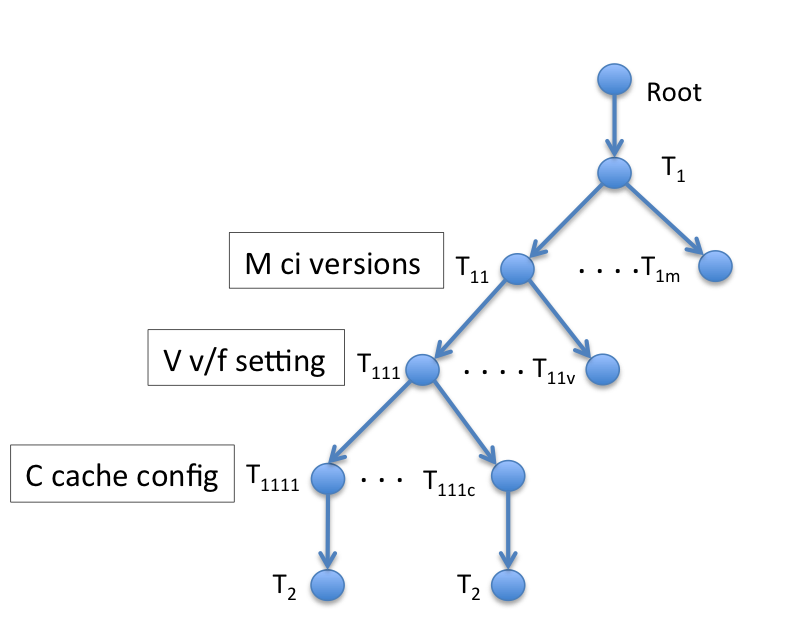
\includegraphics[width=0.36\textwidth]{branch.png}
\label{fig:bnb}
\caption {Example of Branching}
\end{figure}

The pseudo code for our branch and bound algorithm is shown in Algorithm
\ref{BnB}. Let $A_c$ and $P_c$ be the area and period constraints
provided as an input.
In each iteration, we map a task to one of the existing PEs (in lines
14-28) or to a new PE (in lines 30-45), and select a set of custom
instructions and voltage/frequency level for it. For a task $T_i$, the
algorithm enumerates all of its possible implementations which are the
combinations of sets of custom instructions, cache configurations and
voltage/frequency levels. And each of the customized versions are further
branched into multiple versions corresponding to different voltage/
frequency settings. For each of these versions, it could be mapped to
one of the already existing PEs or a new PE. And each PE can further
be tailored based on the various cache configuration supported. This
explains our branching technique in searching the entire design space
tree. In lines 19 and 35, the proceduce \textit{calculate\_params}
updates the current estimation of area, period and energy. In Figure
\ref{fig:bnb}, the number of existing PE for the first task $T_1$ is
null.

At level \textit{i} of the search tree, we have a partial solution
explaining the choice of configurations chosen for tasks $T_1,
T_2...T_i$, the voltage/frequency settings and the cache configuration
for each of the PEs already mapped. Let the period and area in the
partial solution space be \textit{period} and \textit{area} respectively.
With this partial solution, we can prune the subtree based on the
violation of any of the following constraints:

\begin{enumerate}
\item Pruning based on area constraint: By mapping only the software
only version of the remaining tasks in the existing PEs, the total area
occupied on-chip is still equal to \textit{area}. This is because the
software only version of the tasks does not occupy any extra area. If
this \textit{area} violates the area constraint, it is safe to prune the
entire subtree. For example, 

\item Pruning based on period constraint: By mapping the version of the
remaining tasks that has the minimal steady state execution time, the
lower bound of the new period can be estimated to be the \begin{math}
max(period_i, max(E_{i+1},..E_{N}))\end{math}. If the new period violates
the period contraint, it is safe to prune the entire subtree. For
example,

\item Pruning based on Lower Bound Cost (LBC): The LBC is defined as the
lowest possible energy consumption estimated at the level \textit{i}. For
each of the task, we identify the versions of the task that consume the
minimal energy. Then, the LBC can be estimated by summing the minimal
energy version of the remaining tasks $T_{i+1}, T_{i+2} ... T_{N}$. For
example, consider two tasks $T_i, T_j$ with the lowest steady state
energy consumption as $En_{ss,i}, En_{ss,j}$ respectively.
\begin{equation}
LBC = En_{ss,i} + En_{ss,j}
\end{equation}
The estimated LBC indirectly represents that the tasks are mapped to a
dedicated PE. If the more than one task is mapped to a single PE, the
energy consumed is definitely greater than or equal to the sum of the
steady state energy consumption of the individual tasks. If the tasks
$T_i, T_j$ were to be mapped in a single PE, then
\begin{equation}
\label{eq:lb}
LBC \leq En_{ss,i,j}
\end{equation}
From Equation \ref{eq:lb}, it is evident LBC estimated is indeed the
lowest possible energy acheivable in the subtree. One can easily prune a
subtree, if the existing best solution is smaller than the estimated LBC
for the energy.
\end{enumerate}


\begin{algorithm}
\caption{Branch and Bound algorithm}\label{BnB}
\begin{algorithmic}[1]
\State \begin{math} tasks = \lbrace T_1, T_2 ... T_N \rbrace \end{math};
\State $map = [ ]$; 
\State $currA = 0$; \Comment{current area}
\State $currP = 0$; \Comment{current period}
\State $currE = 0$; \Comment{current energy}
\State $existingPEs = \{\}$; \Comment{The set containing existing PEs}
\State
\State $BnB(tasks, A_c, P_c, map, existingPEs);$
\State
\Procedure{BnB}{$tasks, A_c, P_c, map, existingPEs$}
\State
\State $prune(tasks, A_c)$; \Comment{prunning based on the area}
\State $prune(tasks, P_c)$;\Comment{prunning based on the period}
\State $prune(tasks, best\_solution)$; \Comment{prunning based on the LBC}
\State
\If{$tasks \ne null$}  
\State $\backslash\ast$ mapping to one of the existing PEs $\ast\backslash$
\State T = remove a task from $tasks$;
\State
\For{j = 1 to M } \Comment{CIS versions}
\For{k = 1 to V } \Comment{V/F settings}
\For{ each PE in ex\_pe }
\State Add $T_{ijk}$ to map\{PE\};
\State $(currA, currP, currE)$=cal\_params(map($PE$));
\State
\If {$period \leq P_c$ \&\& $area \leq A_c$} 
\State $BnB(tasks, A_c, P_c, map, existingPEs)$;
\Else
\State update $(currA, currP, currE)$ to previous value;
\State Remove $T_{ijk}$ from map\{PE\};
\EndIf
\EndFor
\EndFor
\EndFor
\State
\State $\backslash\ast$ mapping to a new PE $\ast\backslash$
\For{j = 1 to M } \Comment{CIS versions}
\For{k = 1 to V } \Comment{V/F settings}
\For{l = 1 to C }  \Comment{C Cache Configs}
\State Add $T_{ijk}$ to map\{$PE_{l}$\};
\State Add $PE_{l}$ to $existingPEs$ ;
\State $(currA, currP, currE)$=cal\_params(map($PE_{l}$));
\State
\If {$period \leq P_c$ \&\& $area \leq A_c$} 
\State $BnB(tasks, A_c, P_c, map, existingPEs)$;
\Else
\State update $(currA, currP, currEn)$ to previous value;
\State Remove $T_{ijk}$ from map{$PE_{l}$};
\State Remove $PE_{l}$ from $existingPEs$;
\EndIf
\EndFor
\EndFor
\EndFor
\State

\Else 
\State $\backslash\ast$ We have a solution $\ast\backslash$
\State Update the best solution
 \EndIf
\State
\EndProcedure
\end{algorithmic}
\end{algorithm}
   